\documentclass[a4paper,oneside,DIV=10,12pt]{scrartcl}

\usepackage{float}

\usepackage{fontspec}
\setmainfont{STIX Two Text}
\setsansfont{Roboto}
\setmonofont{PT Mono}

\usepackage{microtype}

\usepackage{amsmath}
\usepackage{unicode-math}
\setmathfont{STIX Two Math}

\usepackage{polyglossia}
\setmainlanguage{ukrainian}

\usepackage{graphicx}

\usepackage{booktabs}
\usepackage{cellspace}
\setlength\cellspacetoplimit{2pt}
\setlength\cellspacebottomlimit{2pt}

\usepackage{subcaption}

\usepackage{siunitx}
\sisetup{output-decimal-marker = {,}}

\newcommand\schel[1]{\textit{#1}}

\newcommand\hexword[1]{\texttt{#1}}

\newcommand\barneg[1]{\overline{#1}}

\begin{document}
	\begin{titlepage}
	\begin{center}
		Міністерство освіти і науки України\\
		Національний авіаційний університет\\
		Навчально-науковий інститут комп'ютерних інформаційних технологій\\
		Кафедра комп'ютеризованих систем управління

		\vspace{\fill}
		Лабораторна робота №5\\
		з дисципліни «Комп'ютерна електроніка»\\
		на тему «Дослідження тригерів»\\
		Варіант №3
		
		\vspace{\fill}
		\begin{flushright}
		Виконав:\\
		студент ННІКІТ СП-225\\
		Клокун Владислав\\
		Перевірив:\\
		Андрєєв О. В.
		\end{flushright}
		
		Київ 2017
	\end{center}
	\end{titlepage}
	
	\section{Мета та основні завдання роботи}
		\begin{enumerate}
			\item Вивчення принципів побудови й логіки роботи тригерів на інтегральних мікросхемах.
			\item Вивчення умовно-графічних позначень тригерів.
			\item Освоєння методики дослідження асинхронних і синхронних тригерів у статичному й динамічному режимах.
			\item Вивчення УГЗ, законів функціонування і принципу дії RS-, JK- і~D-тригерів.
		\end{enumerate}
	
	\section{Обладнання та прилади}
		До лабораторної установки входять:
		\begin{enumerate}
			\item RS-, JK- і~D-тригери.
			\item Два вольтметра постійної напруги для виміру значень вихідних напруг, відповідних логічним «0» і~«1».
			\item Індикатори логічних рівнів.
			\item Генератор слів.
			\item Логічний аналізатор.
			\item Набір схем для дослідження логічних елементів в статичному і динамічному режимах.
		\end{enumerate}
		
	\section{Хід роботи}
		\subsection{Дослідження асинхронного RS-тригера}
			Готуємо віртуальну установку (рис.~\ref{fig:rs-flipflop-functioning-law-schematic}) до роботи. Для цього перемикачі \schel{SA1} \schel{SA2} встановлюємо у нижнє положення, при якому вхідні змінні $S$ і~$R$ дорівнюють $0$. Вмикаємо установку на моделювання. Перевіряємо всі набори таблиці істинності. Вимикаємо моделювання.
			
			\begin{figure}[!htbp]
			\centering
				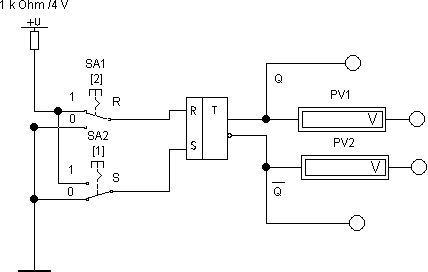
\includegraphics[height=50mm]{assets/01-01-rs-flipflop-functioning-law-schematic.png}
			\caption{Схема віртуальної лабораторної установки для перевірки закону функціонування асинхронного RS-тригера}
			\label{fig:rs-flipflop-functioning-law-schematic}
			\end{figure}
			
			% 0 — 14.910 millivolt
			% 1 —  2.495 volt
			\begin{table}[!htbp]
			\centering
				\begin{tabular}{
					S[table-number-alignment = center, table-format=1.3]
					S[table-number-alignment = center, table-format=1.3]
					S[table-number-alignment = center, table-format=1.3]
					S[table-number-alignment = center, table-format=1.3]
					S[table-number-alignment = center, table-format=1.3]
				}
					\toprule
						{$R$ (\si{\volt})} & {$S$ (\si{\volt})} & {$Q_t$ (\si{\volt})} & {$Q_{t+1}$ (\si{\volt})} & {$\barneg{Q_{t+1}}$ (\si{\volt})}\\
					\midrule
						0.015 & 0.015 & 0.015 & 0.015 & 2.496\\
						0.015 & 0.015 & 2.495 & 2.496 & 0.015\\
						0.015 & 2.495 & 0.015 & 2.496 & 0.015\\
						0.015 & 2.495 & 2.495 & 2.496 & 0.015\\
						2.495 & 0.015 & 0.015 & 0.015 & 2.496\\
						2.495 & 0.015 & 2.495 & 0.015 & 2.496\\
						2.495 & 2.495 & 0.015 & 0.015 & 0.015\\
						2.495 & 2.495 & 2.495 & 0.015 & 0.015\\
					\bottomrule
				\end{tabular}
			\caption{Таблиця істинності асинхронного RS-тригера}
			\label{tab:rs-flipflop-functioning-law-truth-table}
			\end{table}
			
			Досліджуємо RS-тригер у динамічному режимі. Для цього використовуємо схему на рис.~\ref{fig:rs-flipflop-dynamic-mode-schematic}, до якої входять асинхронний RS-тригер, генератор слів і логічний аналізатор.
			
			Налаштовуємо генератор слів. Для цього встановлюємо параметри, наведені у табл.~\ref{tab:rs-flipflop-word-generator-settings}.
			
			\begin{figure}[!htbp]
			\centering
				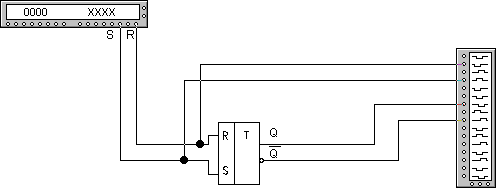
\includegraphics[height=50mm]{assets/01-02-rs-flipflop-dynamic-mode-schematic.png}
			\caption{Схема віртуальної лабораторної установки для дослідження асинхронного RS-тригера в динамічному режимі}
			\label{fig:rs-flipflop-dynamic-mode-schematic}
			\end{figure}
			
			\begin{table}[!htbp]
			\centering
				\begin{tabular}{lr}
					\toprule
						Параметр & Значення\\
					\midrule
						Режим & Step\\
						Trigger & Internal\\
						Фронт & Передній (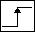
\includegraphics[height = 1em]{assets/front-setting-button.png})\\
						Frequency & 150~Hz\\
						Набір слів & \hexword{000A}\\
						           & \hexword{000E}\\
						           & \hexword{0101}\\
						           & \hexword{0101}\\
						           & \hexword{000E}\\
						           & \hexword{000E}\\
					\bottomrule
				\end{tabular}
			\caption{Налаштування генератора слів для дослідження асинхронного RS-тригера}
			\label{tab:rs-flipflop-word-generator-settings}
			\end{table}
			
			Вмикаємо схему на моделювання. За результатами моделювання будуємо часову діаграму RS-тригера (рис.~\ref{fig:rs-flipflop-dynamic-mode-plot}) та таблицю його переходів (табл.~\ref{tab:rs-flipflop-excitation-table}).
			
			\begin{figure}[!htbp]
			\centering
				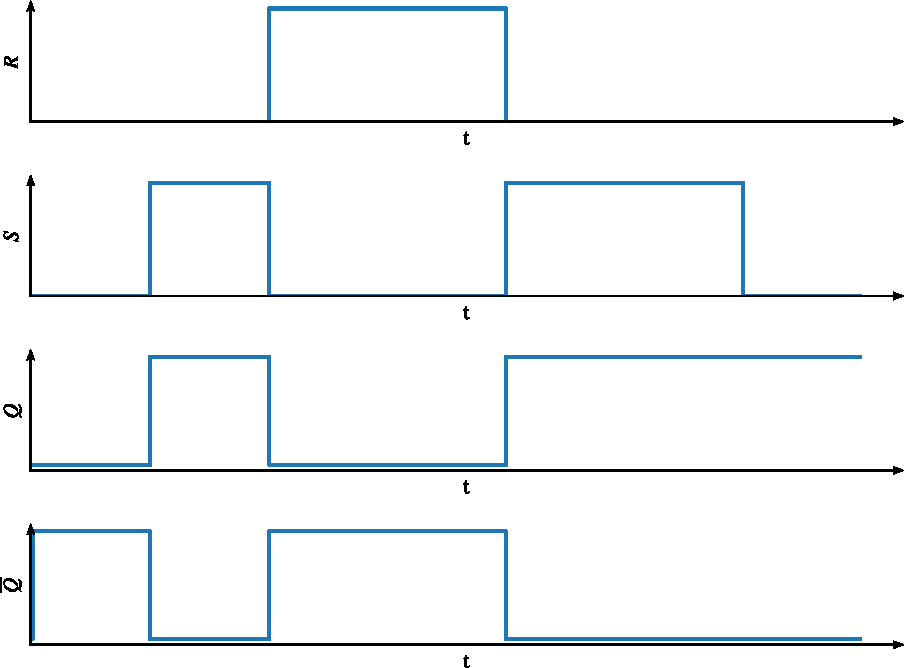
\includegraphics[width = \textwidth]{plots/02-pdf/01-rs-edited.pdf}
			\caption{Часова діаграма асинхронного RS-тригера}
			\label{fig:rs-flipflop-dynamic-mode-plot}
			\end{figure}
			
			\begin{table}[!htbp]
			\centering
				\begin{tabular}{cccc}
					\toprule
						$R$ & $S$ & $Q_t$ & $Q_{t + 1}$\\
					\midrule
						0 & 0 & 0 & 0\\
						0 & 0 & 1 & 1\\
						0 & 1 & 0 & 1\\
						0 & 1 & 1 & 1\\
						1 & 0 & 0 & 0\\
						1 & 0 & 1 & 0\\
						1 & 1 & 0 & —\\
						1 & 1 & 1 & —\\
					\bottomrule
				\end{tabular}
			\caption{Таблиця переходів асинхронного RS-тригера}
			\label{tab:rs-flipflop-excitation-table}
			\end{table}
			
		\subsection{Дослідження синхронного RS-тригера}
			Перевіряємо закон функціонування синхронного RS-тригера за допомогою віртуальної лабораторної установки (рис.~\ref{fig:rsc-flipflop-functioning-law-schematic}). Отримані дані наведені у табл.~\ref{tab:rsc-flipflop-functioning-law-truth-table}
			
			\begin{figure}[!htbp]
			\centering
				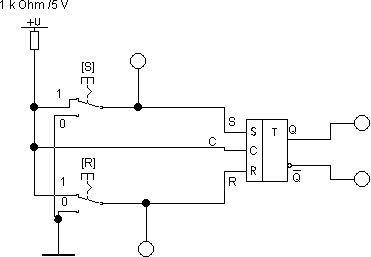
\includegraphics[height=50mm]{assets/02-01-rs-sync-flipflop-functioning-law-schematic.png}
			\caption{Схема віртуальної лабораторної установки для перевірки закону функціонування синхронного RS-тригера}
			\label{fig:rsc-flipflop-functioning-law-schematic}
			\end{figure}
			
			% 0 — 14.910 millivolt
			% 1 —  2.495 volt
			\begin{table}[!htbp]
			\centering
				\begin{tabular}{
					S[table-number-alignment = center, table-format=1.3]
					S[table-number-alignment = center, table-format=1.3]
					S[table-number-alignment = center, table-format=1.3]
					S[table-number-alignment = center, table-format=1.3]
					S[table-number-alignment = center, table-format=1.3]
					S[table-number-alignment = center, table-format=1.3]
				}
					\toprule
						{$C$ (\si{\volt})} & {$R$ (\si{\volt})} & {$S$ (\si{\volt})} & {$Q_t$ (\si{\volt})} & {$Q_{t+1}$ (\si{\volt})} & {$\barneg{Q_{t+1}}$ (\si{\volt})}\\
					\midrule
						2.495 & 0.015 & 0.015 & 0.015 & 0.015 & 2.496\\
						2.495 & 0.015 & 0.015 & 2.495 & 2.496 & 0.015\\
						2.495 & 0.015 & 2.495 & 0.015 & 2.496 & 0.015\\
						2.495 & 0.015 & 2.495 & 2.495 & 2.496 & 0.015\\
						2.495 & 2.495 & 0.015 & 0.015 & 0.015 & 2.496\\
						2.495 & 2.495 & 0.015 & 2.495 & 0.015 & 2.496\\
						2.495 & 2.495 & 2.495 & 0.015 & 0.015 & 0.015\\
						2.495 & 2.495 & 2.495 & 2.495 & 0.015 & 0.015\\
					\bottomrule
				\end{tabular}
			\caption{Таблиця істинності синхронного RS-тригера}
			\label{tab:rsc-flipflop-functioning-law-truth-table}
			\end{table}
			
			Досліджуємо RS-тригер у динамічному режимі. Для цього використовуємо схему на рис.~\ref{fig:rsc-flipflop-dynamic-mode-schematic}, до якої входять синхронний RS-тригер, генератор слів і логічний аналізатор.
			
			Налаштовуємо генератор слів. Для цього встановлюємо параметри, наведені у табл.~\ref{tab:rsc-flipflop-word-generator-settings}.
			
			\begin{table}[!htbp]
			\centering
				\begin{tabular}{lr}
					\toprule
						Параметр & Значення\\
					\midrule
						Режим & Step\\
						Trigger & Internal\\
						Фронт & Передній (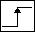
\includegraphics[height = 1em]{assets/front-setting-button.png})\\
						Frequency & 150~Hz\\
						Набір слів & \hexword{000E}\\
						           & \hexword{0101}\\
						           & \hexword{000A}\\
						           & \hexword{000E}\\
						           & \hexword{000A}\\
						           & \hexword{0101}\\
					\bottomrule
				\end{tabular}
			\caption{Налаштування генератора слів для дослідження синхронного RS-тригера}
			\label{tab:rsc-flipflop-word-generator-settings}
			\end{table}
			
			\begin{figure}[!htbp]
			\centering
				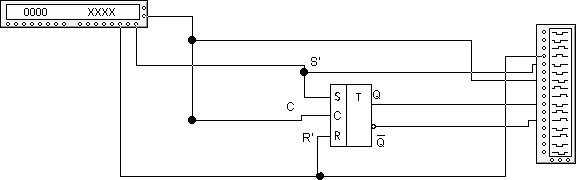
\includegraphics[width = \textwidth]{assets/02-02-rs-sync-flipflop-dynamic-mode-schematic.png}
			\caption{Схема віртуальної лабораторної установки для дослідження синхронного RS-тригера в динамічному режимі}
			\label{fig:rsc-flipflop-dynamic-mode-schematic}
			\end{figure}
			
			Вмикаємо схему на моделювання. За результатами моделювання будуємо часову діаграму RS-тригера (рис.~\ref{fig:rsc-flipflop-dynamic-mode-plot}) та таблицю його переходів (табл.~\ref{tab:rsc-flipflop-excitation-table}).
			
			\begin{figure}[!htbp]
			\centering
				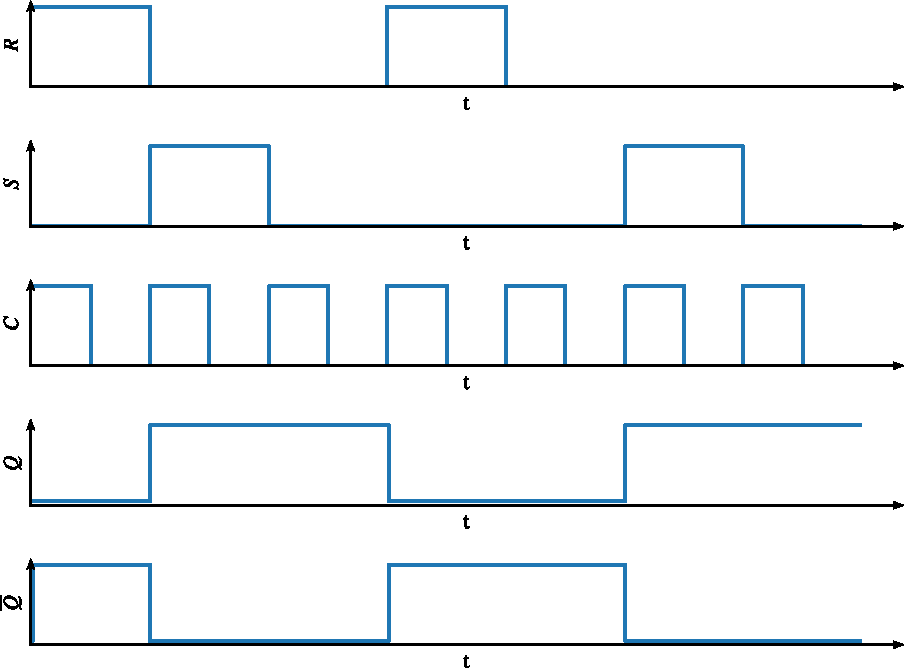
\includegraphics[width = \textwidth]{plots/02-pdf/02-rsc-edited.pdf}
			\caption{Часова діаграма синхронного RS-тригера}
			\label{fig:rsc-flipflop-dynamic-mode-plot}
			\end{figure}
			
			\begin{table}[!htbp]
			\centering
				\begin{tabular}{ccccc}
					\toprule
						$C$ & $R$ & $S$ & $Q_t$ & $Q_{t + 1}$\\
					\midrule
						% 0 & 0 & 0 & 0 & 0\\
						% 0 & 0 & 0 & 1 & 1\\
						% 0 & 0 & 1 & 0 & 0\\
						% 0 & 0 & 1 & 1 & 1\\
						% 0 & 1 & 0 & 0 & 0\\
						% 0 & 1 & 0 & 1 & 1\\
						% 0 & 1 & 1 & 0 & 0\\
						% 0 & 1 & 1 & 1 & 0\\
						1 & 0 & 0 & 0 & 0\\
						1 & 0 & 0 & 1 & 1\\
						1 & 0 & 1 & 0 & 1\\
						1 & 0 & 1 & 1 & 1\\
						1 & 1 & 0 & 0 & 0\\
						1 & 1 & 0 & 1 & 0\\
						1 & 1 & 1 & 0 & —\\
						1 & 1 & 1 & 1 & —\\
					\bottomrule
				\end{tabular}
			\caption{Таблиця переходів синхронного RS-тригера}
			\label{tab:rsc-flipflop-excitation-table}
			\end{table}
			
		\subsection{Дослідження синхронного JK-тригера}
			Перевіряємо закон функціонування JK-тригера за допомогою віртуальної лабораторної установки (рис.~\ref{fig:jk-sync-flipflop-functioning-law-schematic}). Отримані дані наведені у табл.~\ref{tab:jk-flipflop-functioning-law-truth-table}.
			
			\begin{figure}[!htbp]
			\centering
				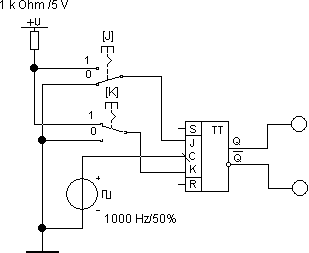
\includegraphics[height = 50mm]{assets/03-01-jk-flipflop-functioning-law-schematic.png}
			\caption{Схема віртуальної лабораторної установки для перевірки закону функціонування синхронного JK-тригера}
			\label{fig:jk-sync-flipflop-functioning-law-schematic}
			\end{figure}
			
			\begin{table}[!htbp]
			\centering
				\begin{tabular}{
					S[table-number-alignment = center, table-format=1.3]
					S[table-number-alignment = center, table-format=1.3]
					S[table-number-alignment = center, table-format=1.3]
					S[table-number-alignment = center, table-format=1.3]
					S[table-number-alignment = center, table-format=1.3]
					S[table-number-alignment = center, table-format=1.3]
				}
					\toprule
						{$C$ (\si{\volt})} & {$J$ (\si{\volt})} & {$K$ (\si{\volt})} & {$Q_t$ (\si{\volt})} & {$Q_{t + 1}$ (\si{\volt})} \\
					\midrule
						2.495 & 0.015 & 0.015 & 0.015 & 0.015 \\
						2.495 & 0.015 & 0.015 & 2.495 & 2.495 \\
						2.495 & 0.015 & 2.495 & 0.015 & 0.015 \\
						2.495 & 0.015 & 2.495 & 2.495 & 0.015 \\
						2.495 & 2.495 & 0.015 & 0.015 & 2.495 \\
						2.495 & 2.495 & 0.015 & 2.495 & 2.495 \\
						2.495 & 2.495 & 2.495 & 0.015 & 2.495 \\
						2.495 & 2.495 & 2.495 & 2.495 & 0.015 \\
					\bottomrule
				\end{tabular}
			\caption{Таблиця істинності синхронного JK-тригера}
			\label{tab:jk-flipflop-functioning-law-truth-table}
			\end{table}
			
			Досліджуємо JK-тригер у динамічному режимі. Для цього використовуємо схему на рис.~\ref{fig:jk-sync-flipflop-dynamic-mode-schematic}, до якої входять синхронний JK-тригер, генератор слів і логічний аналізатор. Також налаштовуємо генератор слів. Для цього встановлюємо параметри, наведені у табл.~\ref{tab:jk-sync-flipflop-word-generator-settings}. Вмикаємо схему на моделювання. За результатами моделювання будуємо часову діаграму синхронного JK-тригера~(рис.~\ref{fig:jk-sync-flipflop-dynamic-mode-time-diagram}) та таблицю переходів (табл.~\ref{tab:jk-sync-flipflop-dynamic-mode-truth-table}).
			
			\begin{figure}[!htbp]
			\centering
				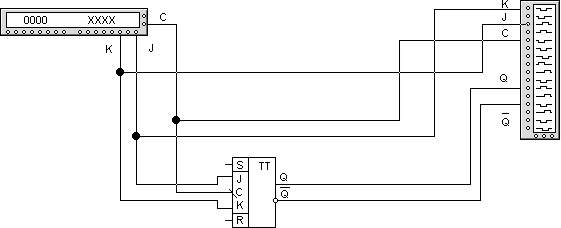
\includegraphics[height = 50mm]{assets/03-02-jk-flipflop-dynamic-mode-schematic.png}
			\caption{Схема віртуальної лабораторної установки для дослідження синхронного JK-тригера в динамічному режимі}
			\label{fig:jk-sync-flipflop-dynamic-mode-schematic}
			\end{figure}
			
			\begin{table}[!htbp]
			\centering
				\begin{tabular}{lr}
					\toprule
						Параметр & Значення\\
					\midrule
						Режим & Step\\
						Trigger & Internal\\
						Фронт & Передній (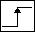
\includegraphics[height=1em]{assets/front-setting-button.png})\\
						Frequency & 150~Hz\\
						Набір слів & \hexword{0101}\\
						           & \hexword{000A}\\
						           & \hexword{000E}\\
						           & \hexword{000A}\\
						           & \hexword{03E7}\\
						           & \hexword{03E7}\\
					\bottomrule
				\end{tabular}
			\caption{Налаштування генератора слів для дослідження синхронного JK-тригера}
			\label{tab:jk-sync-flipflop-word-generator-settings}
			\end{table}
			
			\begin{figure}[!htbp]
			\centering
				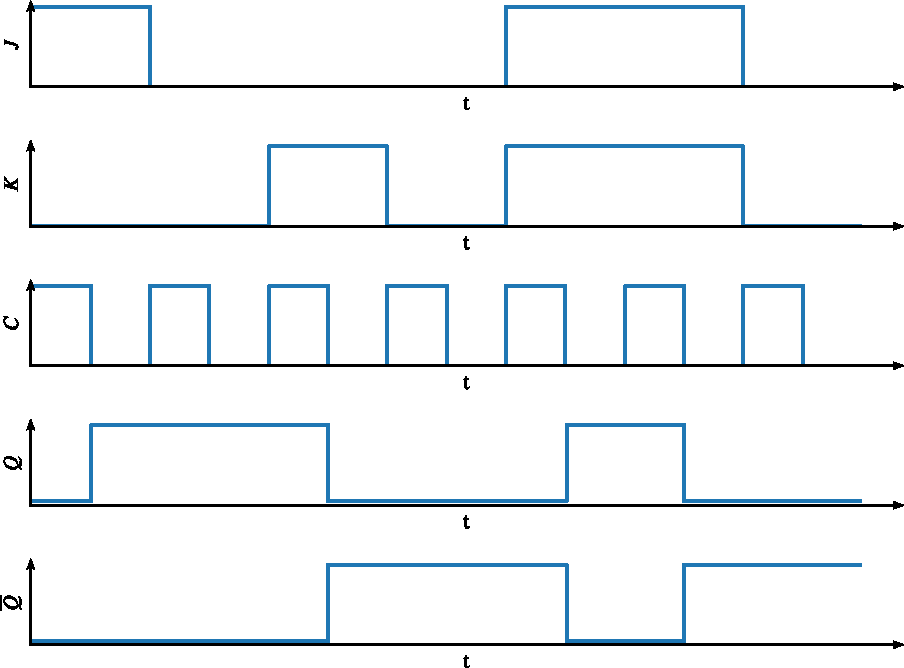
\includegraphics[width = \textwidth]{plots/02-pdf/03-jkc-edited.pdf}
			\caption{Часова діаграма синхронного JK-тригера}
			\label{fig:jk-sync-flipflop-dynamic-mode-time-diagram}
			\end{figure}
			
			\begin{table}[!htbp]
			\centering
			\caption{Таблиця переходів синхронного JK-тригера}
				\begin{tabular}{ccccc}
					\toprule
						$C$ & $J$ & $K$ & $Q_t$ & $Q_{t + 1}$ \\
					\midrule
						1 & 0 & 0 & 0 & 0 \\
						1 & 0 & 0 & 1 & 1 \\
						1 & 0 & 1 & 0 & 0 \\
						1 & 0 & 1 & 1 & 0 \\
						1 & 1 & 0 & 0 & 1 \\
						1 & 1 & 0 & 1 & 1 \\
						1 & 1 & 1 & 0 & 1 \\
						1 & 1 & 1 & 1 & 0 \\
					\bottomrule
				\end{tabular}
			\label{tab:jk-sync-flipflop-dynamic-mode-truth-table}
			\end{table}
			
		\subsection{Дослідження D-тригера з динамічним керуванням}
			Перевіряємо закон функціонування D-тригера за допомогою віртуальної лабораторної установки (рис.~\ref{fig:d-flipflop-functioning-law-schematic}). Отримані дані наведені у табл.~\ref{tab:d-flipflop-functioning-law-truth-table}.
			
			\begin{figure}[!htbp]
			\centering
				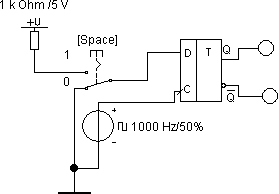
\includegraphics[height = 50mm]{assets/04-01-d-flipflop-functioning-law-schematic.png}
			\caption{Схема віртуальної лабораторної установки для перевірки закону функціонування D-тригера}
			\label{fig:d-flipflop-functioning-law-schematic}
			\end{figure}
			
			\begin{table}[!htbp]
			\centering
				\begin{tabular}{
					S[table-number-alignment = center, table-format=1.3]
					S[table-number-alignment = center, table-format=1.3]
					S[table-number-alignment = center, table-format=1.3]
					S[table-number-alignment = center, table-format=1.3]
				}
					\toprule
						{$C$ (\si{\volt})} & {$D$ (\si{\volt})} & {$Q_t$ (\si{\volt})} & {$Q_{t + 1}$ (\si{\volt})} \\
					\midrule
						2.496 & 0.015 & 0.015 & 0.015\\
						2.496 & 0.015 & 2.496 & 0.015\\
						2.496 & 2.496 & 0.015 & 2.496\\
						2.496 & 2.496 & 2.496 & 2.496\\
					\bottomrule
				\end{tabular}
			\caption{Таблиця істинності D-тригера}
			\label{tab:d-flipflop-functioning-law-truth-table}
			\end{table}
			
			Досліджуємо D-тригер у динамічному режимі. Для цього використовуємо схему на рис.~\ref{fig:d-flipflop-dynamic-mode-schematic}, до якої входять D-тригер, генератор слів і логічний аналізатор. Також налаштовуємо генератор слів. Для цього встановлюємо параметри, наведені у табл.~\ref{tab:d-flipflop-word-generator-settings}. Вмикаємо схему на моделювання. За результатами моделювання будуємо часову діаграму D-тригера~(рис.~\ref{fig:d-flipflop-dynamic-mode-time-diagram}).
			
			\begin{figure}[!htbp]
			\centering
				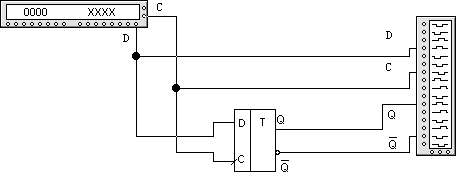
\includegraphics[height = 50mm]{assets/04-02-d-flipflop-dynamic-mode-schematic.png}
			\caption{Схема віртуальної лабораторної установки для дослідження D-тригера в динамічному режимі}
			\label{fig:d-flipflop-dynamic-mode-schematic}
			\end{figure}
			
			\begin{table}[!htbp]
			\centering
				\begin{tabular}{lr}
					\toprule
						Параметр & Значення\\
					\midrule
						Режим & Step\\
						Trigger & Internal\\
						Фронт & Передній (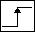
\includegraphics[height=1em]{assets/front-setting-button.png})\\
						Frequency & 150~Hz\\
						Набір слів & \hexword{0101}\\
						           & \hexword{0101}\\
						           & \hexword{000A}\\
						           & \hexword{000A}\\
						           & \hexword{0101}\\
						           & \hexword{0101}\\
					\bottomrule
				\end{tabular}
			\caption{Налаштування генератора слів для дослідження D-тригера}
			\label{tab:d-flipflop-word-generator-settings}
			\end{table}
			
			\begin{figure}[!htbp]
			\centering
				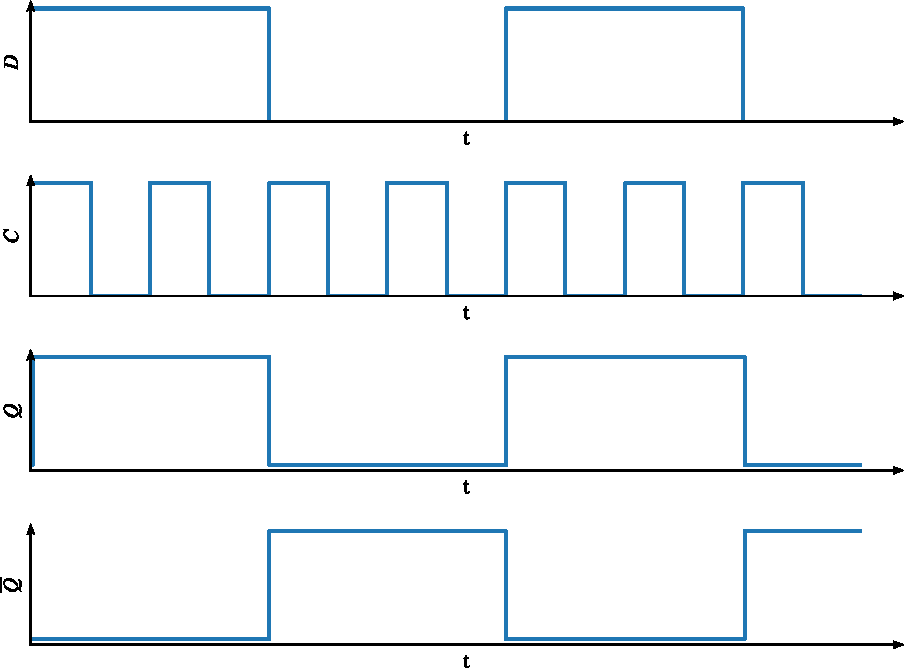
\includegraphics[width = \textwidth]{plots/02-pdf/04-d-edited.pdf}
			\caption{Часова діаграма D-тригера}
			\label{fig:d-flipflop-dynamic-mode-time-diagram}
			\end{figure}
			
			\begin{table}[!htbp]
			\centering
				\begin{tabular}{ccccc}
					\toprule
						$C$ & $D$ & $Q_t$ & $Q_{t + 1}$ \\
					\midrule
						1 & 0 & 0 & 0\\
						1 & 0 & 1 & 0\\
						1 & 1 & 0 & 1\\
						1 & 1 & 1 & 1\\
					\bottomrule
				\end{tabular}
			\caption{Таблиця переходів D-тригера}
			\label{tab:d-flipflop-dynamic-mode-truth-table}
			\end{table}
			
	\section{Висновки}
		Під час виконання даної лабораторної роботи ми вивчили принципи побудови та логіку роботи тригерів на інтегральних мікросхемах; вивчили умовно-графічні позначення тригерів; освоїли методики дослідження асинхронних і~синхронних тригерів у статичному й динамічному режимах; вивчили умовно-графічні позначення, закони функціонування та принципи дії RS-, JK- і~D-тригерів.
		
\end{document}
